%!TEX root = ../../main.tex

\chapter{Stand der Technik}

\section{General Adversarial Network}

\todo[inline,shadow]{Ausreichend mit Quellen hinterlegen...}

Der Begriff GAN \textit{(General Adversarial Network)} ist auf Ian Goodfellow zurückzuführen \cite{gan-original-paper}.
Das Wort bezeichnet ein Konstrukt aus 2 neuronalen Netzen, die sich gegenseitig trainieren.
Durch das spezielle Training gelingt die Generierung von unechten aber realistischen Daten.
Solche Daten können dann zum Beispiel für das Training anderer neuronalen Netze \cite{gan-application-augmenting-training-data}, Bildbearbeitung \cite{gan-application-upscaling, gan-application-blending} und vielen mehr verwendet werden \cite{gan-application-dna-optimizes-protein-functions, gan-application-audio-synthesis}.
\newline

Die beiden Netze eines GANs werden in den Generator und den Discriminator unterschieden.
Aufgabe des Generators ist die Generierung von unechten Daten.
Dafür wandelt er eine zufälligen Eingabe in einen möglichst realistischen Output um.
Die zufällige Eingabe dient dabei als Basis für die Ausgabedaten.
Das ist notwendig, da der Umwandlungsprozess selbst deterministisch ist, aber trotzdem eine Vielzahl an unterschiedlichen Daten generiert werden soll.

Der Output des Generators wird dann vom Discriminator versucht zu falsifizieren.
Dafür wird er sowohl auf die generierten Daten als auch einen Bestand an echten Daten trainiert.
Sein Ziel ist es dann, die falschen Daten des Generators zu identifizieren.
Ziel des Generators hingegen ist es, dass sich der Discriminator irrt und die generierten Daten als echt einstuft.

Ian Goodfellow bezeichnet den Lernprozess auch als Minimax-Spiel, bei die Ausgabe des Discriminators die zu optimierende Größe ist.
Das heißt, der Generator versucht diese zu verkleinern, während der Discriminator sie erhöhen möchte. \cite{gan-minimax} 
\newline

Für diese Arbeit werden zusätzlich Label eingeführt, um die generierten Daten beeinflussen zu können. \todo{noch mehr begründen, wozu Labels gebraucht werden}
Dazu bekommen der Generator und Discriminator das Label als zusätzlichen Input.
So kann der Discriminator aus den echten Daten lernen, dass Daten bei bestimmten Labeln bestimmte Eigenschaften haben.
Dadurch ist dann der Generator gezwungen, diese Eigenschaften zu berücksichtigen, um den Discriminator wieder zu täuschen.
\newline

\todo[inline,shadow]{Bild von GAN zur Erklärung einfügen}


\section{Einfluss von Hyperparametern}
Hyperparameter haben einen sehr großen Einfluss auf das Training.
Der Einfluss reicht so weit, dass bei sehr schlecht gesetzten Parametern das Training keine sinnvollen Resultate mehr erzielt.
Zudem ändern sich die optimalen Hyperparameter bei unterschiedlichen Trainingsdaten oder auch einer anderen Architektur.
Deshalb müssen sie immer wieder neu bestimmt werden.

Obwohl Hyperparameter insgesamt einen großen Einfluss auf die Trainingsresultate haben, ist jedoch nicht jeder Parameter gleich bedeutsam.
Stattdessen sind manche Parameter sehr einflussreich während andere kaum Auswirkung auf das Ergebnis haben.

Zusätzlich ist zu erwähnen, dass Hyperparameter nicht nur das Training beeinflussen sondern auch andere Hyperparameter.
So können manche Parameter in bestimmten Kombinationen stark an Einfluss gewinnen, während andere unwichtiger werden.
Das ist insbesondere bei den Verfahren zur Bestimmung der Hyperparameter ein Problem.
Denn dadurch muss immer eine Kombination getestet und verglichen werden, was deutlich rechenaufwändiger ist, als die Parameter einzeln zu testen.

\section{Verfahren zur Bestimmung von Hyperparametern}
Da Hyperparameter bei jedem neuen neuronalen Netzwerk neu optimiert werden müssen/können, gibt es bereits einige Verfahren zur Bestimmung die im Folgenden erläutert werden.
\newline

\subsection{Manuelle Suche}
Zunächst ist es möglich die Hyperparameter manuell festzulegen.
Zwar wird so sehr viel Rechenaufwand eingespart, da nur eine oder sehr wenige Konfigurationen getestet werden.
Das System ist jedoch sehr aufwändig für die Person, die es konfiguriert.
Zum einen müssen die Werte manuell geändert werden, zum anderen muss eine sehr bedachte Vorauswahl getroffen werden.
Zusätzlich müssen die Ergebnisse auch manuell analysiert werden, um Patterns zu erkennen und so neue Durchläufe zu planen.

\subsection{Gridsearch}
Eine weitere Variante trägt den Namen Gridsearch \cite{hyperparameters-grid-search}.
Bei diesem Verfahren werden für alle gesuchten Hyperparameter mehrere Werte festgelegt.
Es handelt sich also um eine automatisiertere manuelle Suche, die verhältnismäßig einfach zu implementieren ist.
Die verschiedenen Kombinationen werden dann trainiert und die Resultate festgehalten.
Die Suche übernimmt keinerlei Interpretation der Ergebnisse, diese müssen manuell analysiert werden.
Ein Versuch mit der Gridsearch ist somit deutlich rechenaufwändiger als nur ein Parameterset, wie in der manuellen Suche, zu trainieren.
Der exakte Aufwandsunterschied hängt von der festgelegten Anzahl und Variantenreiche der Parameter ab.
Durch die Möglichkeit von Parallelisierung findet die Gridsearch in der Regel bessere Parameter als die sequentielle manuelle Suche in der gleichen Zeit \cite{hyperparameters-random-search}.

\subsection{Random Search}
Die Random Search \cite{hyperparameters-random-search} funktioniert im Training wie die Gridsearch, nur werden zufällige Werte statt dem festgelegten Grid erzeugt.
Die zufälligen Werte haben den Vorteil, dass es weniger Werte-Überlagerungen im Vergleich zur Grid-Kombination gibt.
Deswegen kann die zufällige Suche bei gleich vielen Durchläufen ein größeres Spektrum an Ergebnissen abdecken.
Mittels Automatic Relevance Determination ist es dann möglich, den Einfluss und Wertebereich der einzelnen Hyperparameter darzustellen.

\begin{figure}[H]
	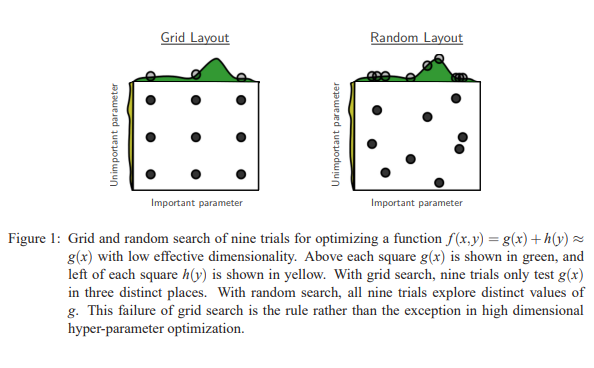
\includegraphics{kapitel/2_stand_der_technik/img/random-vs-grid-search.png}
	\caption{Random Search vs Grid Search (Quelle \cite{hyperparameters-random-search})}
\end{figure}

Problem der Random Search ist vor allem, dass die Räume der guten Hyperparameter sehr klein sind.
Dadurch ist nicht gewährleistet, dass ein zufälliger Wert auch den Raum trifft.
Jedoch erzielen Optimierungen mittels Random Search in der Regel trotzdem gute Ergebnisse.
Dem Grid-Search-Verfahren ist die Random-Search allerdings nicht prinzipiell überlegen \cite{hyperparameters-random-search}.

\subsection{Bayessearch}
\begin{itemize}
	\item Ziel: Anzahl der Versuche reduzieren
	\item Idee: Wiederverwendung von vorherigen Durchläufen
	\item ??
\end{itemize}

\subsection{Zusammenfassung}
In dieser Arbeit wird die Gridsearch zur Anwendung kommen, da sie den besten Kompromiss zwischen benötigter Rechenleistung und Ergebnis bietet.
Das liegt jedoch auch an der zur Verfügung stehenden Hardware.
Bei unbeschränkteren Ressourcen, wären andere Varianten in Betracht zu ziehen.



\section{Related Work}
Es gibt viele verschiedene Versuche und Varianten die Hyperparameter zu optimieren.
Dementsprechend viele Papers und Artikel befassen sich damit.
Einige dieser Arbeiten werden nachfolgend kurz vorgestellt.
\newline

\paragraphNewLine{Best Selection of Generative Adversarial Networks Hyper-Parameters Using Genetic Algorithm \cite{hyperparameters-genetic-algorithm}}
Die Studie befasst sich mit Hyperparameter Optimierung auf Basis von genetischen Algorithmen.
Genetische Algorithmen zeichnen sich unter anderem durch die verwendeten Operatoren Mutation, Kreuzung und Selektion aus \cite{genetic-algorithms}.
Ziel der Studie war es, bestmögliche Hyperparameter für das MNIST Datenset zu finden \cite{dataset:mnist}.
Dabei wurden die Hyperparameter \textit{learning-rate, dropout, batch-size und number of neurons in dense layer} betrachtet.
Ergebnis war eine 100\% Genauigkeit im Vergleich zu 96\% des Vergleichsnetzes.
\newline

Zwar sind die Daten und die Herangehensweise nicht die selbe wie in dieser Arbeit, aber die untersuchten Hyperparameter.
Diese können mit als Basis für die Untersuchung genommen werden.
Zudem verdeutlicht die Arbeit noch einmal die große Auswirkung von Hyperparametern.

\paragraphNewLine{Unsupervised Representation Learning With Deep Convolutional Generative Adversarial Networks \cite{hyperparameters-convolutional-gan}}
Ziel dieser Studie ist es allgemein gute Hyperparameter zu finden.
Dafür wurden Bilder aus verschiedenen Datensets genommen (Large Scale Scene Understanding \cite{dataset:lsun}, Imagenet-1k \cite{dataset:image-net} und einem eigenen Datenset mit Gesichtern).
Bei den Hyperparametern wurden diverse untersucht, zum Beispiel aber nicht ausschließlich die Lernrate, Momentum und Batch-Size.
Im Ergebnis konnten für alle Werte gefunden werden, die über alle Datensets meistens stabil mit zufriedenstellenden Ergebnissen liefen.
\todo{Hyperparameter: learning-rate 0.0002, momentum (beta1) zu 0.5, mini-batch size 128,... (Kapitel 4 Details of adversarial training)}
Erkenntnis der Studie war auch, dass keine Hyperparameter Kombination gefunden werden konnte, die über alle Datensets 100\% stabil laufen konnte.
\newline

Eine allgemeine Studie zum Thema Hyperparameter ist für die Arbeit sehr interessant, da sie gute Ausgangswerte bietet.
Dass keine 100\% stabile Zusammenstellung gefunden werden konnte, verdeutlicht die Notwendigkeit der Feinanpassung an jedes Datenset.


\paragraphNewLine{The GAN Landscape: Losses, Architectures, Regularization, And Normalization \cite{gan-landscape-losses-architectures-regularization-normalization}}
Dieses Studie beschäftigt sich nicht ausschließlich mit Hyperparametertuning.
Aber auch in dieser Studie werden allgemein GANs optimiert und die Erkenntnisse daraus können verwendet werden.
In the GAN Landscape wird das GAN auf die Datensets CIFAR10 \cite{dataset:cifar10}, CELEBA-HQ-128 und LSUN-BEDROOM \cite{dataset:lsun}.
Für das Training wurden dann ein DCGAN und ResNet verglichen.
Dabei fand die Studie viele interssante Erkenntnisse heraus, zum Beispiel eine gute Updatequote von 5:1 zwischen Discriminator und Generator.
\newline

Besonders interessant bei dieser Arbeit ist die Bestimmung von anderen Methoden, wie das unterschiedliche Updaten von Discrimintaor und Generator.
Wieder bietet die Arbeit eine gute Ausgangslage, aber keine Lösung für ein Datenset mit geometrischen Bildern.

\begin{comment}
	
\paragraph{Links}
\begin{itemize}
	\item Inception Score zum Rating von erzeugten Bildern (Salimans et al. 2016)
	\item Frechet Inception Distance (Heusel et al. 2017)
	\item stackoverflow \url{https://stackoverflow.com/questions/46386948/adjusting-gan-hyperparameters}
	\item \url{https://openreview.net/pdf?id=rkGG6s0qKQ}
	\item \url{https://arxiv.org/pdf/1511.06434.pdf%C3%AF%C2%BC%E2%80%B0}
	\item Forget the Learning Rate, Decay Loss \url{https://arxiv.org/ftp/arxiv/papers/1905/1905.00094.pdf}
	\item beste learningRate/Dropout/BatchSize/NumberOfNeuronsInDenseLayer mit evolutionären neuronalen netz für mnist 
	\item zum orientieren ?? \cite{gan-conditional}
\end{itemize}


\end{comment}